\chapter{Courbes intensité--potentiel}\label{ch:b2:current-potential-curves}

On dépose du zinc sur l'acier par électrolyse dans des bains acides. Pourtant, le diagramme E--pH du
volume de première année indique que le zinc, bien au-dessous de la droite du dihydrogène, devrait réduire
l'acide et se dissoudre aussi vite qu'il se dépose. Il n'en est rien, parce qu'un
diagramme dit ce qui peut se produire, non à quelle vitesse. La vitesse d'une réaction d'électrode
est un courant, et tracer ce courant en fonction du potentiel de l'électrode
montre d'emblée quelles réactions sont rapides, lesquelles sont lentes, et lesquelles sont freinées
par l'apport de réactif. Ces \omterm{def:b2:current-potential-curves:ie-curve}{courbes intensité--potentiel} sont l'outil
de tout électrochimiste qui dépose un métal, recharge une batterie ou mesure
le dioxygène d'une rivière.

\begin{recall}
Le volume de première année~: potentiel d'électrode, électrode de référence, relation de
Nernst, diagrammes E--pH et leur limite (ils indiquent ce qui est possible, non à quelle
vitesse). \Cref{ch:b2:cell-thermodynamics}~: $\Delta_r G = -nFE$, la relation de Nernst
démontrée. En physique~: la diffusion et la loi de Fick, $j = -D\,dc/dx$.
\end{recall}

\begin{omfigure}
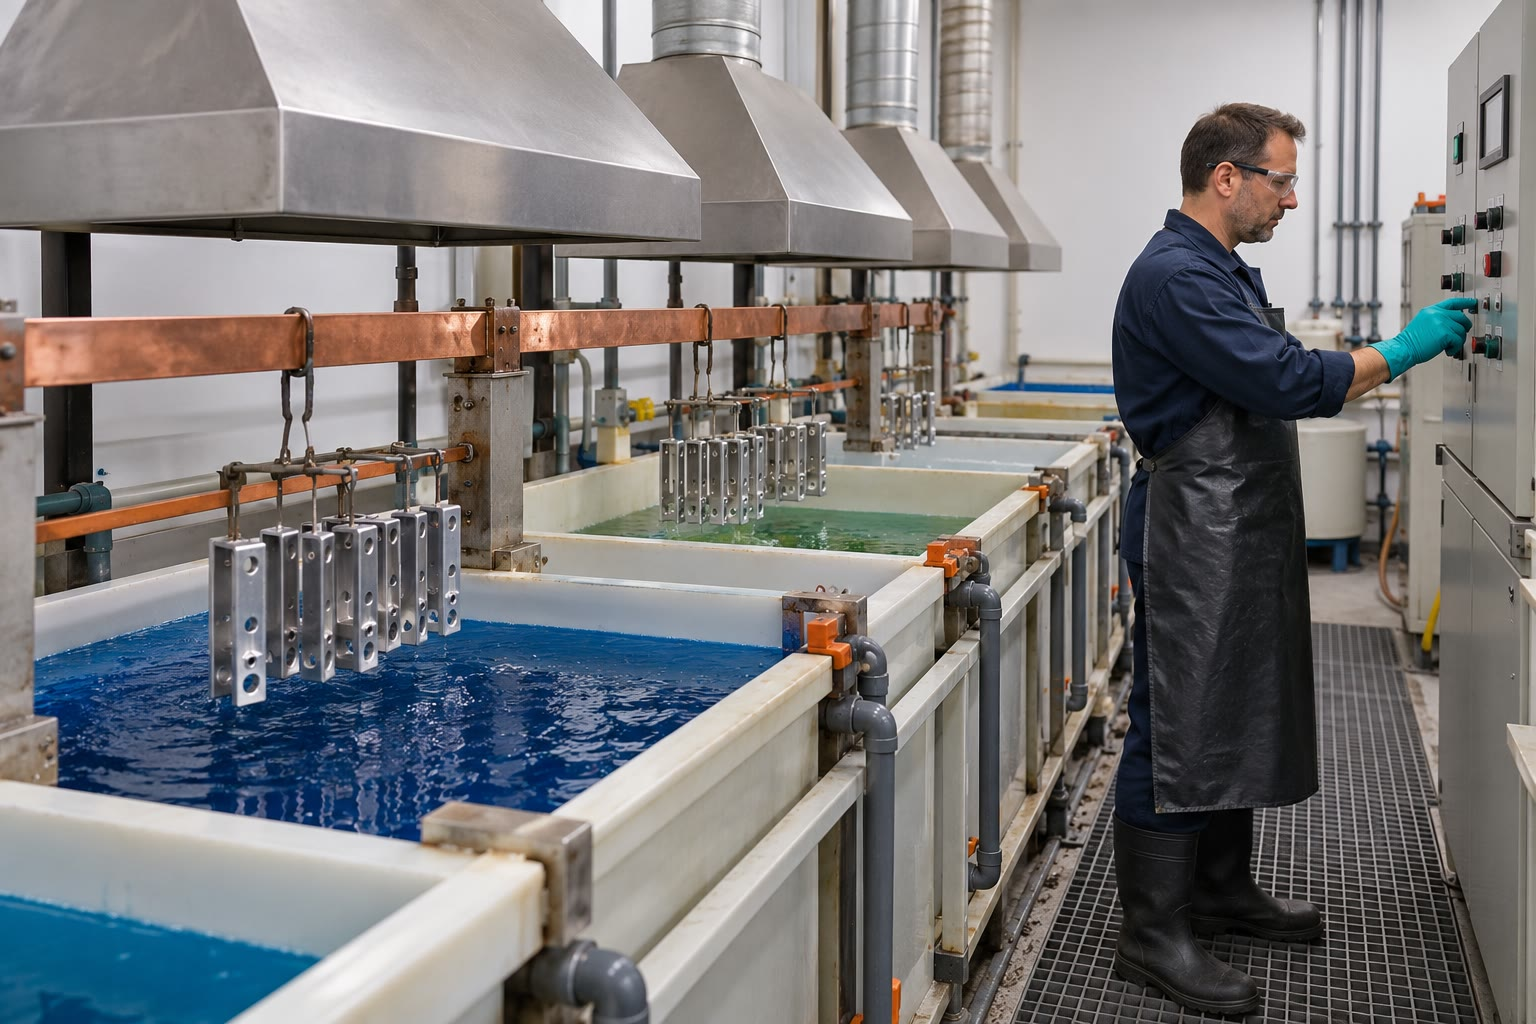
\includegraphics[width=0.62\linewidth]{images/book3/ai/b2-10-electroplating.jpg}

{\small Une chaîne de dépôt électrolytique~: les pièces à revêtir pendent à des barres omnibus en
cuivre, plongées dans les bains, et constituent la cathode~; l'opérateur règle le courant
sur le redresseur. Le courant fixe la vitesse de dépôt du métal~; le potentiel
des pièces décide quel métal, ou quelle quantité de dihydrogène, se forme avec lui.}
\end{omfigure}

\section{Une électrode hors d'équilibre}

\begin{definition}[Courbe intensité--potentiel]\label{def:b2:current-potential-curves:ie-curve}
La \emph{courbe intensité--potentiel}\index{courbe intensite--potentiel@courbe intensité--potentiel} d'une
électrode dans une solution est la représentation du courant $i$ qui traverse l'électrode
en fonction de son potentiel $E$. Un \emph{courant anodique}\index{courant anodique},
compté positivement, correspond à une oxydation à l'électrode~; un
\emph{courant cathodique}\index{courant cathodique}, compté négativement, à une
réduction.
\end{definition}

\begin{definition}[Espèce électroactive]\label{def:b2:current-potential-curves:electroactive}
Une \emph{espèce électroactive}\index{espece electroactive@espèce électroactive} est une espèce
qui peut être oxydée ou réduite à l'électrode dans le domaine de potentiels
considéré.
\end{definition}

\begin{proposition}[Courant et vitesse]\label{prop:b2:current-potential-curves:current-rate}
Si une seule demi-équation à $n$ électrons a lieu à une électrode, le
courant mesure sa vitesse~: $i = nF\,d\xi/dt$, où $\xi$ est l'avancement de
l'oxydation (de sorte que $i > 0$ pour une oxydation, $i < 0$ pour une réduction).
\end{proposition}

\begin{proof}
D'après la \cref{prop:b2:cell-thermodynamics:charge}, un avancement $d\xi$ fait passer la
charge $nF\,d\xi$ à travers l'électrode pendant la durée $dt$.
\end{proof}

Pour enregistrer une telle courbe, il faut imposer et mesurer le potentiel d'une électrode
pendant qu'elle est traversée par un courant --- ce dont une cellule à deux électrodes
est incapable, puisque le courant modifie aussi le potentiel de la seconde
électrode.

\begin{definition}[Montage à trois électrodes]\label{def:b2:current-potential-curves:set-up}
Dans un montage à trois électrodes, le courant circule entre l'\emph{électrode
de travail}\index{electrode de travail@électrode de travail}, celle qu'on étudie, et la \emph{contre-électrode}\index{contre-electrode@contre-électrode},
qui ferme le circuit~; le potentiel
de l'électrode de travail est mesuré par rapport à une électrode de référence que ne traverse
aucun courant. Un potentiostat électronique ajuste le courant pour
que ce potentiel garde la valeur imposée.
\end{definition}

\begin{omfigure}
\begin{tikzpicture}[font=\small, >={Stealth}]
  \pic[transform shape] at (0,0) {beaker={0.7}{omDef!14}};
  \pic at (-0.55,0.25) {electrode={black!35}};
  \pic at (0.55,0.25) {electrode={black!15}};
  \pic (r) at (0.0,0.15) {probe};
  \draw[thick, rounded corners] (-2.2,4.3) rectangle (2.2,5.5);
  \node at (0,4.9) {potentiostat};
  \draw[thick, omThm] (-0.40,2.65) -- (-0.40,3.5) -- (-1.6,3.5) -- (-1.6,4.3);
  \draw[thick, omDef] (0.70,2.65) -- (0.70,3.5) -- (1.6,3.5) -- (1.6,4.3);
  \draw[thick] (r-top) -- (0,4.3);
  \node[anchor=east, font=\scriptsize, omThm] at (-1.65,3.85) {ET};
  \node[anchor=west, font=\scriptsize, omDef] at (1.65,3.85) {CE};
  \node[anchor=west, font=\scriptsize] at (0.05,3.95) {ER};
  \draw[<-, omProp, thick] (-0.75,1.2) -- (-2.0,1.4) node[left, text=black, align=right] {électrode\\ de travail};
  \draw[<-, omProp, thick] (0.85,1.2) -- (2.1,1.4) node[right, text=black, align=left] {contre-\\ électrode};
  \draw[<-, omProp, thick] (0.05,0.5) -- (1.4,-0.4) node[right, text=black] {électrode de référence};
  \node[font=\scriptsize, align=center] at (0,6.0) {impose $E_{\text{ET}} - E_{\text{ER}}$, mesure $i$};
\end{tikzpicture}

{\small Le montage à trois électrodes. Le potentiostat fait circuler le courant
entre l'\omterm{def:b2:current-potential-curves:set-up}{électrode de travail} (ET) et la \omterm{def:b2:current-potential-curves:set-up}{contre-électrode} (CE) de manière à
maintenir le potentiel de l'\omterm{def:b2:current-potential-curves:set-up}{électrode de travail}, mesuré par rapport à l'électrode de
référence (ER), à la valeur imposée~; aucun courant ne traverse la
référence.}
\end{omfigure}

Lorsque aucun courant ne circule et que les deux formes d'un couple sont présentes, l'électrode
prend le potentiel de Nernst du couple --- si l'échange d'électrons est assez rapide
pour l'établir. Écarter le potentiel de cette valeur fait circuler un
courant.

\section{Systèmes rapides et systèmes lents}

\begin{definition}[Surtension]\label{def:b2:current-potential-curves:overpotential}
La \emph{surtension}\index{surtension} d'une électrode traversée par un
courant $i$ est $\eta = E(i) - E_{\text{éq}}$, la différence entre son
potentiel et le potentiel d'équilibre (de Nernst) du couple. Le
\emph{potentiel seuil}\index{potentiel seuil} d'une demi-équation est le
potentiel au-delà duquel son courant devient notable.
\end{definition}

\begin{definition}[Systèmes rapides et lents]\label{def:b2:current-potential-curves:fast-slow}
Un couple est un \emph{système rapide}\index{systeme rapide@système rapide} sur une électrode donnée si un
courant notable circule dès que le potentiel s'écarte de son potentiel de
Nernst~; c'est un \emph{système lent}\index{systeme lent@système lent} s'il faut une \omterm{def:b2:current-potential-curves:overpotential}{surtension} de
quelques dixièmes de volt avant que le courant devienne notable, dans
un sens comme dans l'autre.
\end{definition}

Qu'un système soit rapide ou lent dépend du couple et du matériau de
l'électrode. Les couples \ce{Fe^3+}/\ce{Fe^2+} et \ce{Ag+}/\ce{Ag} sont rapides sur
platine~; la réduction de \ce{H+} est rapide sur platine mais lente sur mercure,
plomb ou zinc~; l'oxydation de l'eau en dioxygène est lente sur toute électrode.
Les transferts d'électrons qui rompent ou forment des liaisons, comme ceux de \ce{O2} ou de \ce{H2},
sont en général lents~; le transfert d'un électron entre deux ions de forme presque
identique est rapide. L'allure de la partie montante d'une courbe lente provient de
la cinétique du transfert électronique, établie dans le volume de troisième année.

\begin{omfigure}
\begin{tikzpicture}
\begin{axis}[omie, width=0.47\linewidth, height=5.4cm, xmin=0.25, xmax=1.3,
  ymin=-1.3, ymax=1.3, xlabel={$E$}, ylabel={$i$}, title={\small système rapide}]
\addplot[omanodic] table[x=E, y=i, restrict expr to domain={\thisrow{i}}{0:2}] {figdata/out/bachelor-2-ie-curves-a.dat};
\addplot[omcathodic] table[x=E, y=i, restrict expr to domain={\thisrow{i}}{-2:0}] {figdata/out/bachelor-2-ie-curves-a.dat};
\draw[densely dotted] (axis cs:0.77,-1.2) -- (axis cs:0.77,1.2);
\node[font=\scriptsize, anchor=north west] at (axis cs:0.78,-0.05) {$E_{\text{éq}}$};
\node[font=\scriptsize, anchor=south] at (axis cs:1.1,1.0) {\ce{Fe^2+} $\to$ \ce{Fe^3+}};
\node[font=\scriptsize, anchor=north] at (axis cs:0.45,-1.0) {\ce{Fe^3+} $\to$ \ce{Fe^2+}};
\end{axis}
\end{tikzpicture}\hfill
\begin{tikzpicture}
\begin{axis}[omie, width=0.47\linewidth, height=5.4cm, xmin=-0.25, xmax=1.8,
  ymin=-1.3, ymax=1.3, xlabel={$E$}, ylabel={$i$}, title={\small système lent}]
\addplot[omanodic] table[x=E, y=i, restrict expr to domain={\thisrow{i}}{0:2}] {figdata/out/bachelor-2-ie-curves-c.dat};
\addplot[omcathodic] table[x=E, y=i, restrict expr to domain={\thisrow{i}}{-2:0}] {figdata/out/bachelor-2-ie-curves-c.dat};
\draw[densely dotted] (axis cs:0.77,-1.2) -- (axis cs:0.77,1.2);
\draw[<->, omProp] (axis cs:0.77,0.5) -- (axis cs:1.12,0.5) node[midway, above, font=\scriptsize] {$\eta_a$};
\draw[<->, omProp] (axis cs:0.42,-0.5) -- (axis cs:0.77,-0.5) node[midway, below, font=\scriptsize] {$\eta_c$};
\node[font=\scriptsize, anchor=north west] at (axis cs:0.78,-0.05) {$E_{\text{éq}}$};
\end{axis}
\end{tikzpicture}

{\small \omterm{def:b2:current-potential-curves:ie-curve}{Courbes intensité--potentiel} modèles d'un couple dont les deux formes sont présentes
à concentrations égales (branche anodique en rouge, cathodique en bleu). À gauche, un \omterm{def:b2:current-potential-curves:fast-slow}{système
rapide}~: le courant change de signe brutalement au potentiel d'équilibre. À droite,
un \omterm{def:b2:current-potential-curves:fast-slow}{système lent}~: aucun courant ne circule sur un domaine de potentiels autour de lui~; chaque
branche exige une \omterm{def:b2:current-potential-curves:overpotential}{surtension}. Les deux atteignent les mêmes paliers limites, fixés par
la diffusion. (Valeurs illustratives.)}
\end{omfigure}

\section{Transport de matière et courants limites}

Lorsque le transfert d'électrons est rapide, le courant est limité par l'arrivée du
réactif à l'électrode. Dans une solution agitée, une mince couche de liquide
au contact de l'électrode reste presque immobile, et le réactif la traverse par
diffusion.

\begin{definition}[Couche de diffusion et courant limite]\label{def:b2:current-potential-curves:limiting-current}
La \emph{couche de diffusion}\index{couche de diffusion} est la couche de solution,
d'épaisseur $\delta$ (de quelques à quelques dizaines de micromètres dans une solution
agitée), au contact de l'électrode, que les espèces traversent uniquement par
diffusion. Le \emph{courant limite}\index{courant limite} est le courant
atteint lorsque l'\omterm{def:b2:current-potential-curves:electroactive}{espèce électroactive} est consommée aussi vite qu'elle arrive, sa
concentration à la surface étant nulle.
\end{definition}

\begin{omfigure}
\begin{tikzpicture}[font=\small, >={Stealth}, x=1.2cm, y=1.2cm]
  \fill[black!25] (-0.4,0) rectangle (0,3);
  \node[rotate=90, font=\scriptsize] at (-0.2,1.5) {électrode};
  \draw[->] (0,0) -- (4.6,0) node[right] {$x$};
  \draw[->] (0,0) -- (0,3.2) node[above] {$c$};
  \draw[densely dashed] (1.6,0) -- (1.6,3);
  \node[below, font=\scriptsize] at (1.6,0) {$\delta$};
  \draw[omDef, thick] (0,1.2) -- (1.6,2.4) -- (4.4,2.4);
  \draw[omThm, thick] (0,0.02) -- (1.6,2.4);
  \node[font=\scriptsize, anchor=west] at (2.6,2.6) {cœur de la solution, $c^b$ (agitée)};
  \node[font=\scriptsize, omDef, anchor=east] at (-0.45,1.2) {$c^s$};
  \node[font=\scriptsize, omThm, anchor=west] at (1.7,0.5) {$c^s = 0$~: courant limite};
  \node[font=\scriptsize, align=center] at (0.8,3.0) {couche de\\ diffusion};
\end{tikzpicture}

{\small Concentration du réactif au voisinage d'une électrode dans une solution
agitée. Dans la \omterm{def:b2:current-potential-curves:limiting-current}{couche de diffusion}, le profil est linéaire~; le flux, donc le
courant, est proportionnel à $c^b - c^s$. Il est maximal lorsque le réactif est
consommé dès qu'il arrive ($c^s = 0$, en rouge).}
\end{omfigure}

\begin{theorem}[Courant limite]\label{thm:b2:current-potential-curves:limiting}
Pour une espèce de concentration $c$ au cœur de la solution et de coefficient de diffusion $D$,
qui traverse une \omterm{def:b2:current-potential-curves:limiting-current}{couche de diffusion} d'épaisseur $\delta$ jusqu'à une électrode de surface $A$,
le \omterm{def:b2:current-potential-curves:limiting-current}{courant limite} vaut, en valeur absolue,
\[
  |i_{\lim}| = \frac{nFADc}{\delta} .
\]
\end{theorem}

\begin{proof}
En régime stationnaire, le profil de concentration dans la couche est linéaire (la seconde
loi de Fick avec $\partial c/\partial t = 0$ donne $d^2c/dx^2 = 0$)~: le flux
vers l'électrode vaut $j = D(c - c^s)/\delta$, en moles par unité de surface et de
temps. Chaque molécule qui arrive réagit avec $n$ électrons~: $|i| = nFAj =
nFAD(c - c^s)/\delta$, maximal pour $c^s = 0$.
\end{proof}

\begin{example}[Ordre de grandeur d'un courant limite]\label{ex:b2:current-potential-curves:ilim}
Pour une espèce à \qty{10}{mmol/L} (\qty{10}{mol/m^3}), avec $D =
\qty{7e-10}{m^2/s}$, $\delta = \qty{20}{\micro m}$, $n = 1$, sur
\qty{1.0}{cm^2}~: $|i_{\lim}| = 96\,485 \times 10^{-4} \times 7 \times 10^{-10}
\times 10/(2 \times 10^{-5}) = \qty{3.4}{mA}$.
\end{example}

\begin{theorem}[Vague d'un système rapide]\label{thm:b2:current-potential-curves:wave}
Pour un couple rapide $\mathrm{Ox} + n\,\mathrm e^- \rightleftharpoons \mathrm{Red}$,
de \omterm{def:b2:current-potential-curves:limiting-current}{courant limite} anodique $i_{\lim,a} > 0$ (fixé par Red) et de \omterm{def:b2:current-potential-curves:limiting-current}{courant limite}
cathodique $i_{\lim,c} < 0$ (fixé par Ox), la courbe en régime stationnaire est
\[
  E = E_{1/2} + \frac{RT}{nF}\ln\frac{i - i_{\lim,c}}{i_{\lim,a} - i},
  \qquad E_{1/2} = E^\circ + \frac{RT}{nF}\ln\frac{D_{\text{Red}}}{D_{\text{Ox}}} ,
\]
l'épaisseur de la couche étant la même pour les deux formes.
\end{theorem}

\begin{proof}
\omterm{def:b2:current-potential-curves:fast-slow}{Système rapide}~: la relation de Nernst est vérifiée à la surface, $E = E^\circ + (RT/nF)
\ln(c^s_{\text{Ox}}/c^s_{\text{Red}})$. Profils linéaires~: un \omterm{def:b2:current-potential-curves:ie-curve}{courant anodique} $i$
consomme Red et produit Ox à la surface, $i = nFAD_{\text{Red}}(c^b_{\text{Red}}
- c^s_{\text{Red}})/\delta = -nFAD_{\text{Ox}}(c^b_{\text{Ox}} - c^s_{\text{Ox}})/\delta$.
Avec $i_{\lim,a} = nFAD_{\text{Red}}c^b_{\text{Red}}/\delta$ et $i_{\lim,c} =
-nFAD_{\text{Ox}}c^b_{\text{Ox}}/\delta$, on obtient $c^s_{\text{Red}} = (i_{\lim,a} -
i)\delta/(nFAD_{\text{Red}})$ et $c^s_{\text{Ox}} = (i - i_{\lim,c})\delta/(nFAD_{\text{Ox}})$.
Il reste à reporter dans la relation de Nernst.
\end{proof}

\begin{corollary}[Potentiel de demi-vague]\label{cor:b2:current-potential-curves:half-wave}
Lorsque les deux formes ont des coefficients de diffusion égaux, $E_{1/2} = E^\circ$~: si
une seule forme est présente, le courant vaut la moitié de sa valeur limite au potentiel
standard du couple.
\end{corollary}

\begin{proof}
Si seul Red est présent, $i_{\lim,c} = 0$, et pour $i = i_{\lim,a}/2$ le logarithme
s'annule~: $E = E_{1/2} = E^\circ$ lorsque $D_{\text{Red}} = D_{\text{Ox}}$.
\end{proof}

\begin{proposition}[Les paliers mesurent des concentrations]\label{prop:b2:current-potential-curves:plateau}
À agitation et électrode fixées, la hauteur d'un palier est proportionnelle à la
concentration de l'espèce qu'il consomme~: une électrode maintenue à un
potentiel situé sur le palier est un capteur ampérométrique.
\end{proposition}

\begin{proof}
$|i_{\lim}| = (nFAD/\delta)\,c$, et le facteur entre parenthèses est constant à agitation
et température fixées.
\end{proof}

\begin{omfigure}
\begin{tikzpicture}
\begin{axis}[omie, width=0.47\linewidth, height=5.0cm, xmin=0.25, xmax=1.3,
  ymin=-0.3, ymax=1.3, xlabel={$E$}, ylabel={$i$}, title={\small \ce{Fe^2+} seul présent}]
\addplot[omanodic] table[x=E, y=i] {figdata/out/bachelor-2-ie-curves-b.dat};
\draw[densely dotted] (axis cs:0.77,0) -- (axis cs:0.77,0.5) -- (axis cs:0.25,0.5);
\node[font=\scriptsize, anchor=north] at (axis cs:0.77,-0.02) {$E_{1/2}$};
\node[font=\scriptsize, anchor=south west] at (axis cs:0.27,0.5) {$i_{\lim}/2$};
\node[font=\scriptsize, anchor=south] at (axis cs:1.12,1.0) {palier};
\end{axis}
\end{tikzpicture}\hfill
\begin{tikzpicture}
\begin{axis}[width=0.42\linewidth, height=5.0cm, xmin=0, xmax=1.05, ymin=0, ymax=1.1,
  axis x line=bottom, axis y line=left, xtick=\empty, ytick=\empty,
  xlabel={$c$}, ylabel={$i_{\lim}$}, label style={font=\small},
  title={\small ampérométrie}]
\addplot[omanodic, mark=*, mark size=1.2pt] table[x=c, y=i] {figdata/out/bachelor-2-ie-curves-e.dat};
\end{axis}
\end{tikzpicture}

{\small À gauche~: la vague d'un couple rapide lorsque seule la forme réduite est présente
(modèle)~; sa mi-hauteur se situe au potentiel de demi-vague. À droite~: la hauteur
du palier croît proportionnellement à la concentration.}
\end{omfigure}

\section{Le solvant et l'électrode}

L'eau est elle-même électroactive~: elle est oxydée en dioxygène
(\ce{2H2O -> O2 + 4H+ + 4e-}) et réduite en dihydrogène (\ce{2H+ + 2e- -> H2}, ou
\ce{2H2O + 2e- -> H2 + 2OH-}). Comme le solvant ne s'épuise jamais, ses courbes
n'ont pas de palier~: elles montent brutalement et bornent toutes les autres courbes.

\begin{definition}[Domaine d'électroactivité]\label{def:b2:current-potential-curves:window}
Les \emph{murs du solvant}\index{mur du solvant} sont les branches abruptes de
l'oxydation et de la réduction du solvant. Le \emph{domaine
d'électroactivité}\index{domaine d'electroactivite@domaine d'électroactivité} est le domaine de potentiels compris entre eux,
dans lequel on peut observer les courbes des espèces dissoutes.
\end{definition}

\begin{proposition}[Le domaine d'électroactivité de l'eau]\label{prop:b2:current-potential-curves:window}
Dans l'eau à un pH donné, le domaine se situe autour du domaine thermodynamique des
deux couples de l'eau, $\qty{0}{V} - 0.059\,\mathrm{pH}$ et $\qty{1.23}{V} -
0.059\,\mathrm{pH}$, élargi de chaque côté par la \omterm{def:b2:current-potential-curves:overpotential}{surtension} de la
réaction correspondante sur l'électrode utilisée.
\end{proposition}

\begin{proof}[Argument]
Chaque mur commence près du potentiel de Nernst de son couple, décalé de la
\omterm{def:b2:current-potential-curves:overpotential}{surtension} seuil~: l'oxydation de l'eau est lente sur toutes les électrodes, si bien que
le mur anodique se situe quelques dixièmes de volt au-dessus de \qty{1.23}{V} (à pH 0)~; la
réduction de \ce{H+} est rapide sur platine, dont le mur cathodique reste proche de
\qty{0}{V}, mais lente sur zinc, plomb ou mercure, dont le mur se situe plusieurs dixièmes de
volt plus bas.
\end{proof}

\begin{omfigure}
\begin{tikzpicture}
\begin{axis}[omie, width=0.82\linewidth, height=5.4cm, xmin=-1.2, xmax=2.0,
  ymin=-3, ymax=3, xlabel={$E$ (V)}, ylabel={$i$}, clip=true, clip mode=individual]
\addplot[omwall] table[x=E, y=i] {figdata/out/bachelor-2-ie-curves-d-high.dat};
\addplot[omcathodic] table[x=E, y=i, restrict expr to domain={\thisrow{E}}{-1.2:0.6}] {figdata/out/bachelor-2-ie-curves-d-Pt.dat};
\addplot[omanodic] table[x=E, y=i, restrict expr to domain={\thisrow{E}}{0.6:2.0}] {figdata/out/bachelor-2-ie-curves-d-Pt.dat};
\draw[densely dotted] (axis cs:0,-2.8) -- (axis cs:0,2.8);
\draw[densely dotted] (axis cs:1.23,-2.8) -- (axis cs:1.23,2.8);
\node[font=\scriptsize, anchor=north west] at (axis cs:0.02,-0.1) {0};
\node[font=\scriptsize, anchor=north west] at (axis cs:1.24,-0.1) {1.23};
\node[font=\scriptsize, omDef, anchor=west] at (axis cs:0.05,-2.2) {\ce{H+} $\to$ \ce{H2} sur Pt};
\node[font=\scriptsize, gray, anchor=east] at (axis cs:-0.85,-1.0) {sur Zn, Pb};
\node[font=\scriptsize, omThm, anchor=east] at (axis cs:1.18,2.2) {\ce{H2O} $\to$ \ce{O2}};
\end{axis}
\end{tikzpicture}

{\small Les murs de l'eau à pH 0 (modèle). La réduction de \ce{H+} commence près de
\qty{0}{V} sur platine (en bleu) mais plusieurs dixièmes de volt plus bas sur des métaux comme
le zinc ou le plomb (en tirets)~; l'oxydation de l'eau exige une \omterm{def:b2:current-potential-curves:overpotential}{surtension} sur toute
électrode. Le \omterm{def:b2:current-potential-curves:window}{domaine d'électroactivité} est l'intervalle compris entre les murs.}
\end{omfigure}

\section{Lire des courbes}

\begin{method}[Tracer l'allure des courbes d'une solution]\label{met:b2:current-potential-curves:sketch-ie}
\begin{enumerate}
  \item Tracer les deux \omterm{def:b2:current-potential-curves:window}{murs du solvant} pour le pH et le matériau de
        l'électrode.
  \item Pour chaque couple présent, placer son potentiel de Nernst (les deux formes
        présentes) ou $E^\circ$ (une seule forme)~: un \omterm{def:b2:current-potential-curves:fast-slow}{système rapide} y coupe l'axe
        brutalement~; un \omterm{def:b2:current-potential-curves:fast-slow}{système lent} est décalé de ses \omterm{def:b2:current-potential-curves:overpotential}{surtensions}.
  \item Donner à chaque vague un palier proportionnel à la concentration de
        l'espèce qu'elle consomme~; une électrode métallique qui s'oxyde elle-même n'a pas de
        palier (le métal ne s'épuise pas).
  \item Additionner les courants des réactions possibles à chaque potentiel.
\end{enumerate}
\end{method}

\begin{method}[Lire les courbes]\label{met:b2:current-potential-curves:read-ie}
\begin{enumerate}
  \item À potentiel imposé, lire sur chaque courbe le courant de chaque
        réaction~: elles se déroulent simultanément, en proportion de leurs courants.
  \item À courant imposé (électrolyse), chercher le potentiel auquel les courbes
        anodiques ou cathodiques totalisent ce courant~; les réactions en jeu
        sont celles dont les courbes y contribuent.
  \item Pour une pile, ou pour un métal qui se corrode, le \omterm{def:b2:current-potential-curves:ie-curve}{courant anodique} d'une réaction
        est égal au \omterm{def:b2:current-potential-curves:ie-curve}{courant cathodique} de l'autre~: chercher ce couple de
        points.
\end{enumerate}
\end{method}

\begin{example}[Le dépôt de zinc en bain acide]\label{ex:b2:current-potential-curves:zinc}
Dans un bain de zinc acide, la cathode est le siège de deux réductions possibles~: \ce{Zn^2+
+ 2e- -> Zn} ($E^\circ = \qty{-0.76}{V}$, \omterm{def:b2:current-potential-curves:fast-slow}{système rapide}) et \ce{2H+ + 2e- -> H2}
($E^\circ = \qty{0}{V}$). Thermodynamiquement, le dihydrogène devrait se former d'abord et le zinc
jamais. Mais sur zinc, la réduction de \ce{H+} est lente~: son mur se situe au-dessous de
\qty{-0.76}{V}, et au potentiel où le zinc se dépose à une vitesse utile,
il se forme peu de dihydrogène. C'est la courbe, non le diagramme, qui explique le
dépôt.
\end{example}

\begin{history}[La polarographie]
\begin{minipage}[t]{0.25\linewidth}
\vspace{0pt}
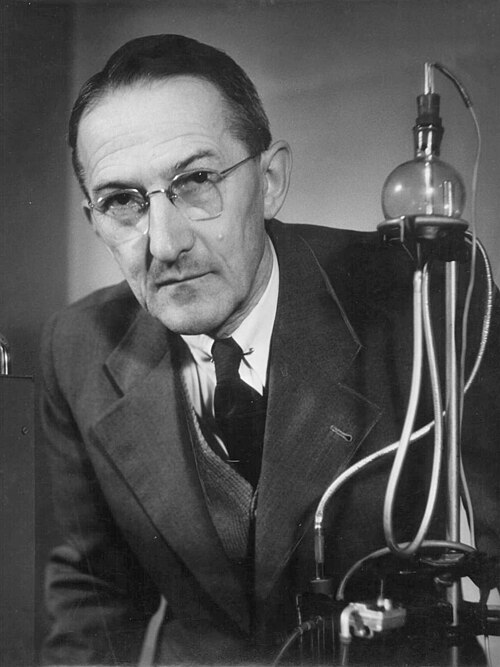
\includegraphics[width=\linewidth]{images/book3/heyrovsky.jpg}
\end{minipage}\hfill
\begin{minipage}[t]{0.71\linewidth}
\vspace{0pt}
En 1922, Jaroslav Heyrovský enregistra le courant traversant une électrode de mercure
qui se formait goutte après goutte à l'extrémité d'un capillaire, pendant que l'on balayait
le potentiel~: chaque espèce réductible donnait une marche dont la position l'identifiait et
dont la hauteur mesurait sa concentration. Le renouvellement de la goutte gardait la surface
fraîche, et la forte \omterm{def:b2:current-potential-curves:overpotential}{surtension} du dihydrogène sur le mercure ouvrait un large domaine
cathodique. La polarographie lui valut le prix Nobel de chimie en 1959
et fonda la chimie électroanalytique~; la photographie le montre avec une
électrode à goutte de mercure. (Photographie~: archives de l'Institut J.~Heyrovský
de chimie physique, CC BY-SA 3.0, Wikimedia Commons.)
\end{minipage}
\end{history}

\section{Exercices}

\begin{exercise}[$\star$]\label{exo:b2:current-potential-curves:1}
Dans une pile Daniell qui débite un courant, donner le signe du courant à
l'électrode de zinc et à l'électrode de cuivre, avec les conventions de ce
chapitre.
\end{exercise}

\begin{exercise}[$\star$]\label{exo:b2:current-potential-curves:2}
Calculer le \omterm{def:b2:current-potential-curves:limiting-current}{courant limite} de réduction de \ce{Ag+} (\qty{2.0}{mmol/L}, $D =
\qty{1.6e-9}{m^2/s}$) sur \qty{0.50}{cm^2} avec $\delta = \qty{25}{\micro m}$
(valeurs d'un modèle).
\end{exercise}

\begin{exercise}[$\star$]\label{exo:b2:current-potential-curves:3}
Sur les courbes modèles du chapitre, comment reconnaît-on un \omterm{def:b2:current-potential-curves:fast-slow}{système rapide} et un \omterm{def:b2:current-potential-curves:fast-slow}{système
lent}~? Donner un exemple de chaque sur platine.
\end{exercise}

\begin{exercise}[$\star$]\label{exo:b2:current-potential-curves:4}
Une solution ne contient que \ce{Fe^2+}. À quel potentiel son \omterm{def:b2:current-potential-curves:ie-curve}{courant anodique}
atteint-il la moitié de son palier, si les deux formes diffusent de la même façon ($E^\circ = \qty{0.77}{V}$)~?
\end{exercise}

\begin{exercise}[$\star\star$]\label{exo:b2:current-potential-curves:5}
Une électrode de platine plongeant dans une solution de \ce{Fe^3+} et de \ce{Cu^2+} (concentrations
égales, $E^\circ$ = 0.77 et \qty{0.34}{V}) est balayée vers les potentiels
négatifs. Décrire la courbe~: vagues, paliers, leurs hauteurs, et le mur
cathodique.
\end{exercise}

\begin{exercise}[$\star\star$]\label{exo:b2:current-potential-curves:6}
Dans la solution de l'\cref{exo:b2:current-potential-curves:5}, le potentiel de
l'électrode est maintenu à \qty{0.50}{V}, puis à \qty{0.10}{V}. Que se passe-t-il dans
chaque cas~?
\end{exercise}

\begin{exercise}[$\star\star$]\label{exo:b2:current-potential-curves:7}
Donner les potentiels de Nernst des deux couples de l'eau à pH 0 et à pH 14, et
tracer l'allure du déplacement du \omterm{def:b2:current-potential-curves:window}{domaine d'électroactivité} sur platine avec le pH.
\end{exercise}

\begin{exercise}[$\star\star$]\label{exo:b2:current-potential-curves:8}
On titre \ce{Fe^2+} par \ce{Ce^4+} pendant qu'une électrode de platine maintenue à
\qty{1.0}{V} enregistre le courant. Tracer l'allure du courant en fonction du volume ajouté
et expliquer comment il permet de repérer l'équivalence (\ce{Ce^4+}/\ce{Ce^3+}~: $E^\circ =
\qty{1.72}{V}$).
\end{exercise}

\begin{exercise}[$\star\star$]\label{exo:b2:current-potential-curves:9}
Doubler la vitesse d'agitation divise par deux l'épaisseur de la \omterm{def:b2:current-potential-curves:limiting-current}{couche de diffusion}. Qu'advient-il
des paliers, du potentiel de demi-vague et du potentiel à courant
nul d'un \omterm{def:b2:current-potential-curves:fast-slow}{système rapide}~?
\end{exercise}

\begin{exercise}[$\star\star\star$]\label{exo:b2:current-potential-curves:10}
Établir l'équation de la vague d'un \omterm{def:b2:current-potential-curves:fast-slow}{système rapide} lorsque seul Red est présent, et
montrer que le tracé de $E$ en fonction de $\log[i/(i_{\lim} - i)]$ est une droite de
pente $0.059/n$ volt à \qty{25}{\degreeCelsius}.
\end{exercise}

\begin{exercise}[$\star\star\star$]\label{exo:b2:current-potential-curves:11}
Un morceau de zinc plongé dans un acide à \qty{1}{mol/L} ne se dissout que lentement, alors que
le même morceau en contact avec un fil de platine se dissout vite, avec un dégagement de dihydrogène
sur le platine. Expliquer à l'aide des \omterm{def:b2:current-potential-curves:ie-curve}{courbes intensité--potentiel}.
\end{exercise}

\begin{exercise}[$\star\star\star$]\label{exo:b2:current-potential-curves:12}
Pour oxyder une espèce dont la vague se situe à \qty{2.0}{V} à pH 0, faudrait-il choisir une
électrode de platine ou une électrode à forte \omterm{def:b2:current-potential-curves:overpotential}{surtension} de dioxygène~? Expliquer, et dire
ce qui se formerait sinon.
\end{exercise}

\section{Problème~: une sonde à oxygène pour une rivière}

\begin{problem}[{Problème du week-end --- la cathode d'un capteur ampérométrique de
dioxygène, le courant limite à travers sa membrane, l'étalonnage dans
une eau saturée d'air avec la loi de Henry, et la teneur en dioxygène d'une rivière}]
\label{pb:b2:current-potential-curves:1}
Une sonde ampérométrique à oxygène comporte une cathode en or et une anode en argent dans un
gel de chlorure de potassium, séparés de l'échantillon par une fine membrane perméable aux
gaz. La cathode est maintenue à \qty{-0.60}{V} par rapport à l'anode argent--chlorure
d'argent. Données à \qty{25}{\degreeCelsius}~: constante de la \omterm{prop:b2:chemical-potential:henry}{loi de Henry} de
\ce{O2}, $H = \qty{1.3e-5}{mol/(m^3.Pa)}$~; pression de vapeur de l'eau
\qty{3.17}{kPa}~; dioxygène dans l'air sec 20.95~\% en volume~; $E^\circ(\ce{O2}/\ce{H2O}) =
\qty{1.229}{V}$~; $E^\circ(\ce{AgCl}/\ce{Ag}) = \qty{0.222}{V}$. Membrane (valeurs
d'un modèle)~: surface \qty{0.10}{cm^2}, épaisseur \qty{25}{\micro m}, coefficient de
diffusion effectif de \ce{O2} à travers elle \qty{1.0e-10}{m^2/s}.
% ledger: henry:O2, pvap:H2O.298, air:O2, dfg:Cl-_ao, dfg:AgCl_cr, aw:O

\medskip
\noindent\textbf{Partie I --- La cathode.}
\begin{enumerate}
  \item Écrire la réduction du dioxygène en milieu neutre.
  \item Écrire la réaction à l'anode d'argent, ainsi que la réaction globale.
  \item Calculer le potentiel de Nernst du couple \ce{O2}/\ce{H2O} à pH 7 avec
        $p_{\ce{O2}} = \qty{0.21}{bar}$.
  \item Exprimer le potentiel de la cathode, \qty{-0.60}{V} par rapport à Ag/AgCl, sur
        l'échelle de l'hydrogène, en prenant égale à 1 l'activité des ions chlorure du gel.
  \item Pourquoi faut-il maintenir la cathode bien au-dessous du potentiel de Nernst de
        \ce{O2}~?
  \item Pourquoi choisit-on un potentiel situé sur le palier~?
  \item Qu'est-ce qui fixe la limite inférieure des potentiels utilisables~?
\end{enumerate}

\medskip
\noindent\textbf{Partie II --- Le \omterm{def:b2:current-potential-curves:limiting-current}{courant limite}.}
\begin{enumerate}[resume]
  \item Décrire le profil de concentration de \ce{O2} à travers la membrane lorsque la
        cathode fonctionne sur son palier.
  \item Écrire le flux de \ce{O2} à travers la membrane.
  \item En déduire le courant en fonction de la concentration $c$ du \ce{O2}
        dissous.
  \item Pourquoi utilise-t-on l'épaisseur de la membrane à la place de la \omterm{def:b2:current-potential-curves:limiting-current}{couche de diffusion}~?
  \item Pourquoi la mesure dépend-elle peu de l'agitation de la rivière, mais
        beaucoup de l'encrassement de la membrane~?
\end{enumerate}

\medskip
\noindent\textbf{Partie III --- L'étalonnage.}
\begin{enumerate}[resume]
  \item Calculer la pression partielle de \ce{O2} au-dessus d'une eau saturée d'air sous
        \qty{1.013}{bar} et à \qty{25}{\degreeCelsius}.
  \item Calculer la concentration du \ce{O2} dissous à saturation, en
        \unit{mol/m^3}.
  \item L'exprimer en \unit{mg/L}.
  \item Prévoir le courant de la sonde dans une eau saturée d'air.
  \item La sonde indique en réalité \qty{4.05}{\micro A} dans une eau saturée d'air
        (données de l'exercice). Calculer sa sensibilité en \unit{\micro A} par
        \unit{mg/L}.
  \item Pourquoi étalonner plutôt que se fier au courant prévu~?
  \item Que devrait indiquer la sonde dans une eau débarrassée de son dioxygène~?
\end{enumerate}

\medskip
\noindent\textbf{Partie IV --- La rivière.}
\begin{enumerate}[resume]
  \item Dans un échantillon de rivière à \qty{25}{\degreeCelsius}, la sonde indique
        \qty{2.80}{\micro A}. Calculer le dioxygène dissous en \unit{mg/L}.
  \item L'exprimer en pourcentage de la saturation.
  \item L'eau d'une rivière est presque saturée en dioxygène à sa source.
        Proposer une cause à ce déficit.
  \item Quelle quantité de \ce{O2} la sonde consomme-t-elle en une heure~? Perturbe-t-elle
        l'échantillon~?
  \item Pourquoi faut-il refaire l'étalonnage si la rivière est à
        \qty{15}{\degreeCelsius}~?
  \item Donner la concentration en dioxygène dissous de l'échantillon.
\end{enumerate}
\end{problem}
